\section{5th Sheaf Cobordism}
Suppose we have a punctured Riemann sphere $M$ and $\Lambda_0^0$, $\Lambda_0^\infty$, $\Lambda_0^{squig}$, a nested regions $U\subset U' \subset M$, and a chart $f : U \rightarrow \R^2$ such that $U'$ maps to $R:=(-1,1)_x \times (-n-1,2)_z$ under $f$
\begin{itemize}
\item $\Lambda_0^0$ gets mapped to $\{(x,z)\in R \mid z=1\}$, co-oriented upward.

\item $\Lambda_0^\infty$ gets mapped to $\overset{n}{\underset{k=1}{\cup}}\{(x,z)\in R \mid z=-k\}$, co-oriented downward.

\item $\Lambda_0^{squig}$ gets mapped to $\{(x,z)\in R \mid x=0\}$, co-oriented towards the left.
\end{itemize}
and a sheaf defined by the following squiggly legible diagram. All the maps corresponding to blue strands are $\iota_1$ and the red strands $\iota_0$ otherwise stated. I have omitted these maps from the diagram.\\

\begin{figure}[H]
    \centering
    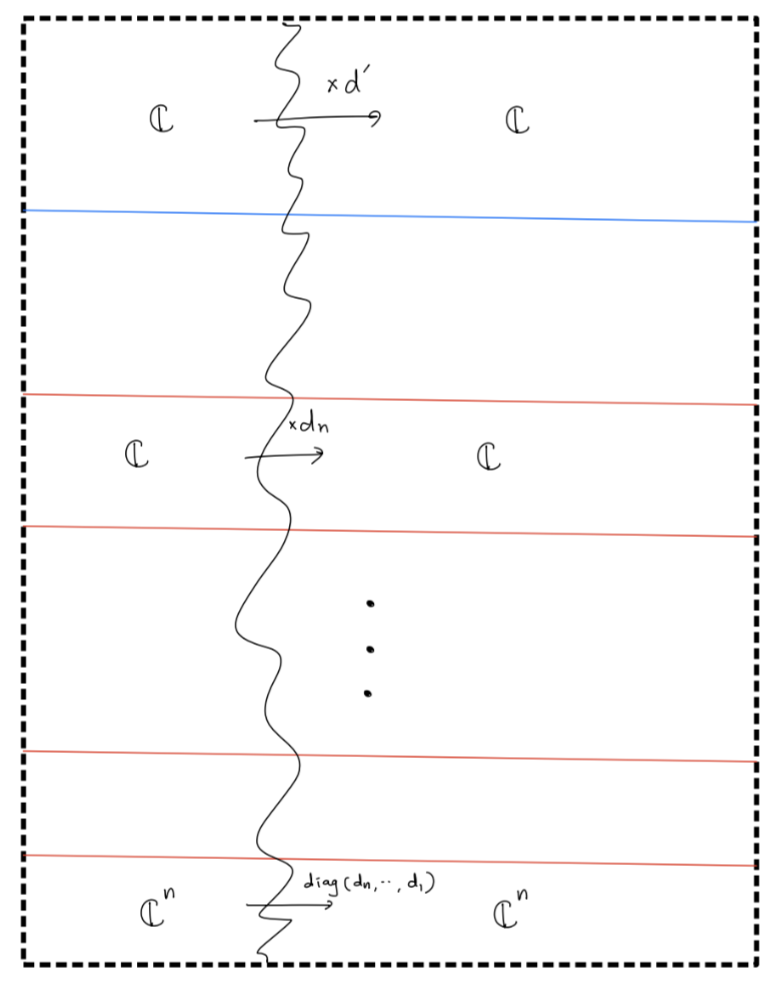
\includegraphics[scale = 0.95]{diagrams/cobord5/1.png} 
    \caption{}
    \label{fig:your-label}
\end{figure}

Then we define a cobordism starting from the above sheaf, say $cobord_5(n)$ supported on $U$. At the end of the cobordism , the sheaf, under the same chart $f$, is described as the following squiggly legible diagram. 

\begin{figure}[H]
    \centering
    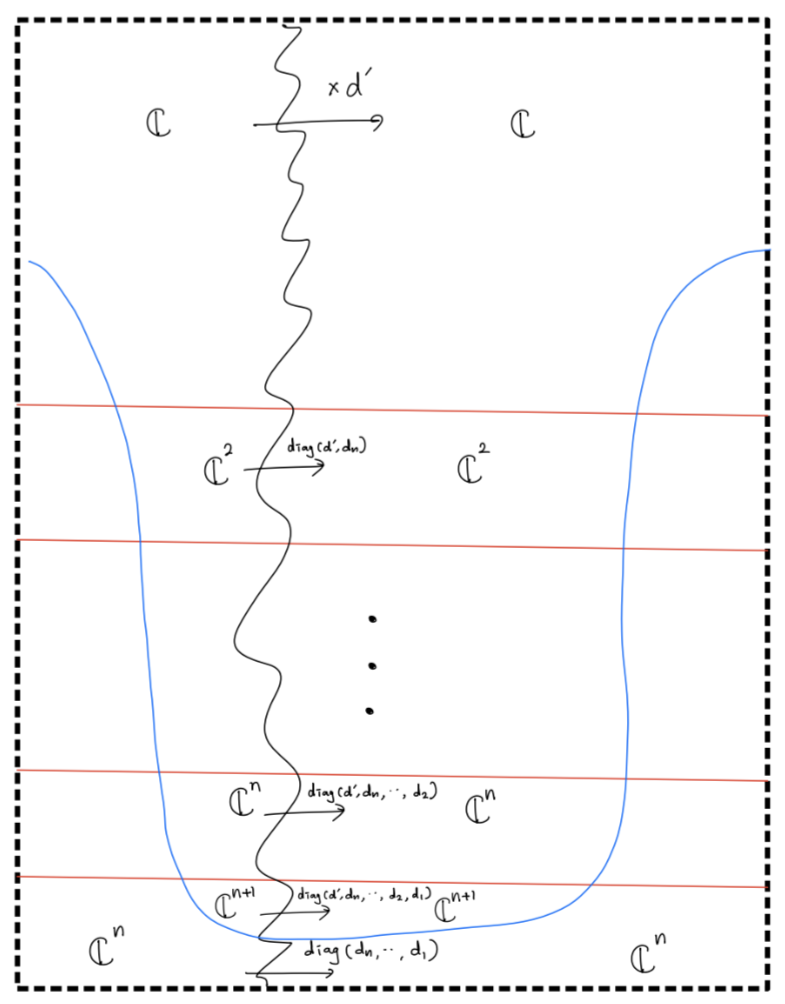
\includegraphics[scale = 0.95]{diagrams/cobord5/7.png} 
    \caption{}
    \label{fig:your-label}
\end{figure}

We define $cobord_5(n)$ inductively as follows.
\begin{enumerate}[label = (\roman*)]
\item For $n=1$, we define $cobord_5(1)$ to be $cobord_1$ from
\begin{figure}[H]
    \centering
    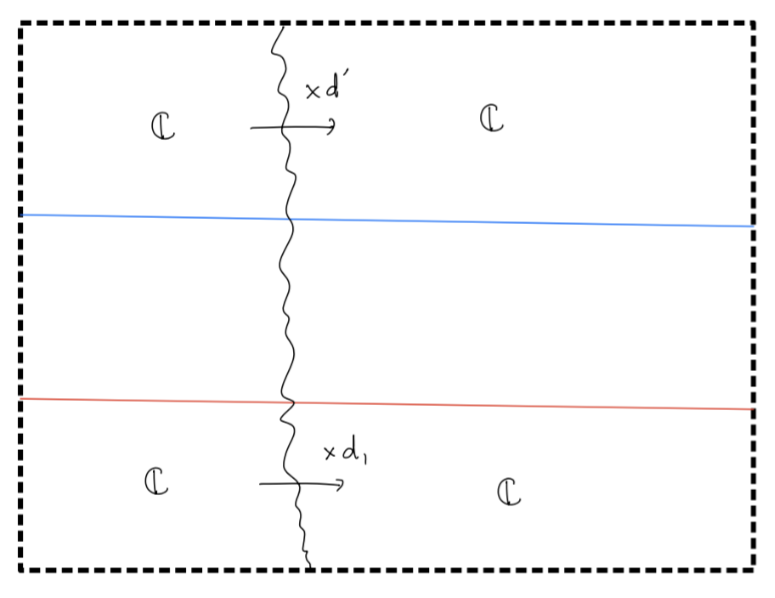
\includegraphics[scale = 0.8]{diagrams/cobord5/2.png} 
    \caption{}
    \label{fig:your-label}
\end{figure}
to
\begin{figure}[H]
    \centering
    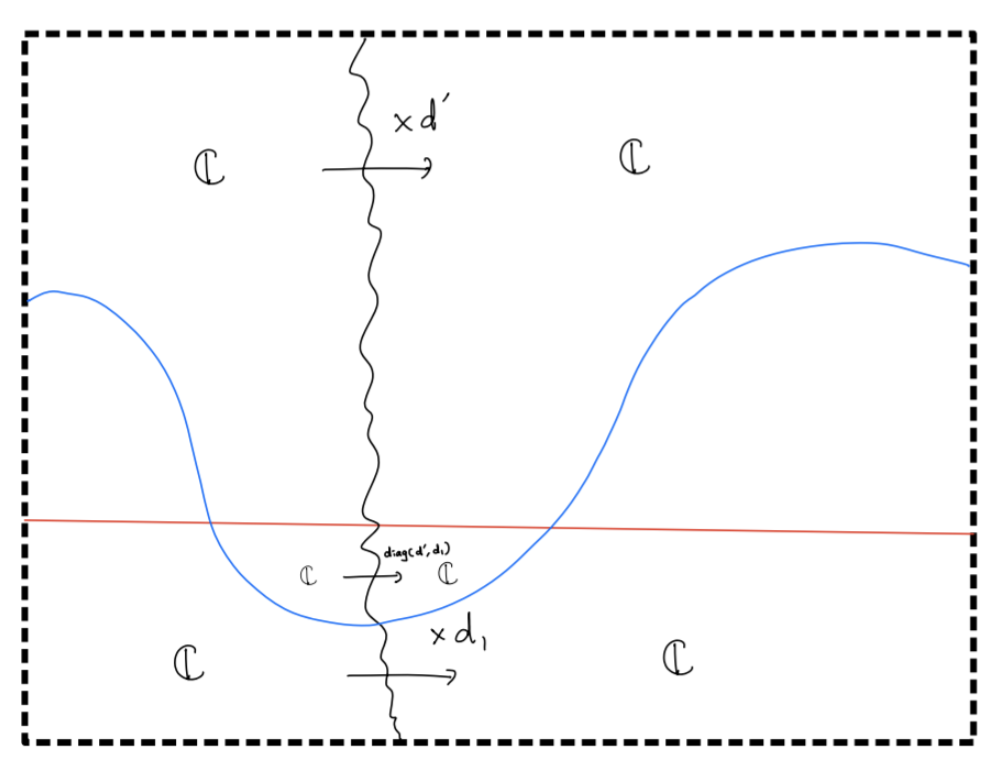
\includegraphics[scale = 0.6]{diagrams/cobord5/3.png} 
    \caption{}
    \label{fig:your-label}
\end{figure}

\item For $n>0$,
\begin{enumerate}[label = (Step \arabic*)]
\item we first apply $cobord_5(n-1)$ to the square region surrounded by a purple dotted line.

\begin{figure}[H]
    \centering
    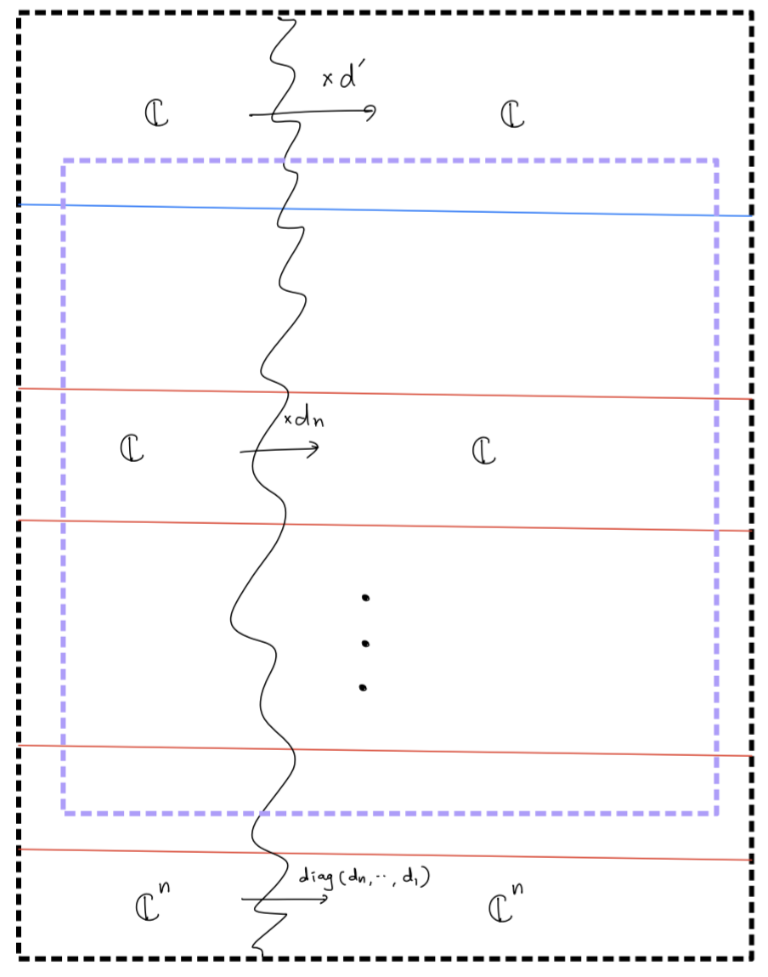
\includegraphics[scale = 0.95]{diagrams/cobord5/4.png} 
    \caption{}
    \label{fig:your-label}
\end{figure}

by induction hypothesis, we get

\begin{figure}[H]
    \centering
    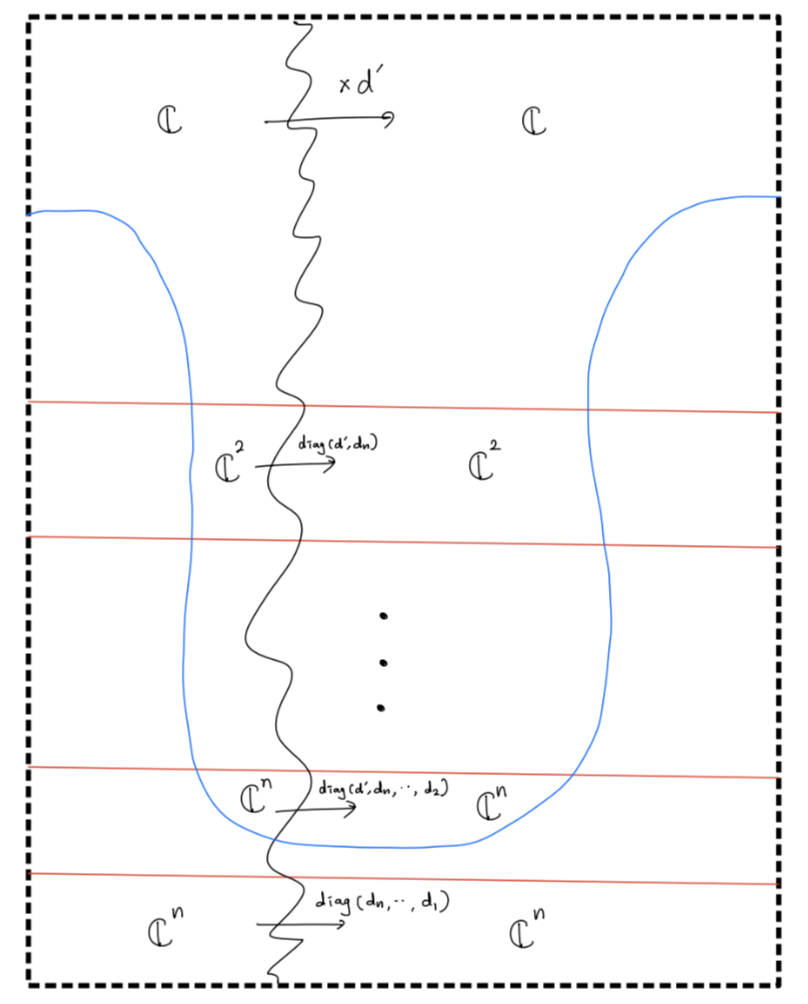
\includegraphics[scale = 0.95]{diagrams/cobord5/5.png}
    \caption{}
    \label{fig:your-label}
\end{figure}

\item apply $cobord_1$ to the square region surrounded by purple dotted lines.

\begin{figure}[H]
    \centering
    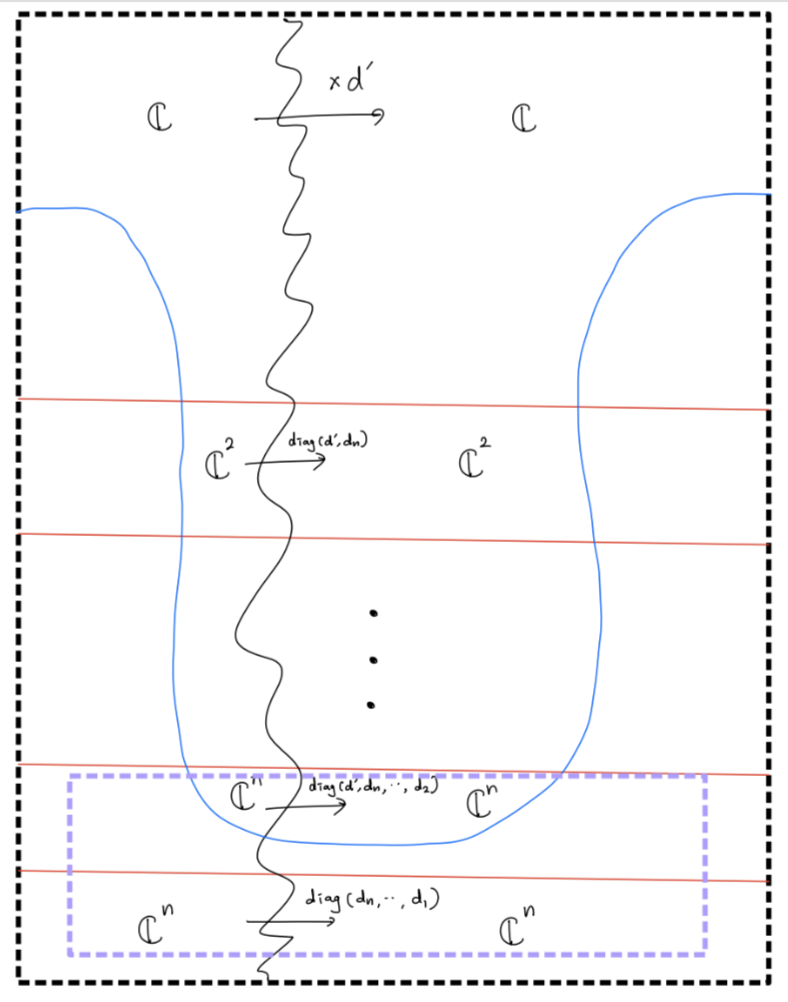
\includegraphics[scale = 0.95]{diagrams/cobord5/6.png}
    \caption{}
    \label{fig:your-label}
\end{figure}

we get the final sheaf

\begin{figure}[H]
    \centering
    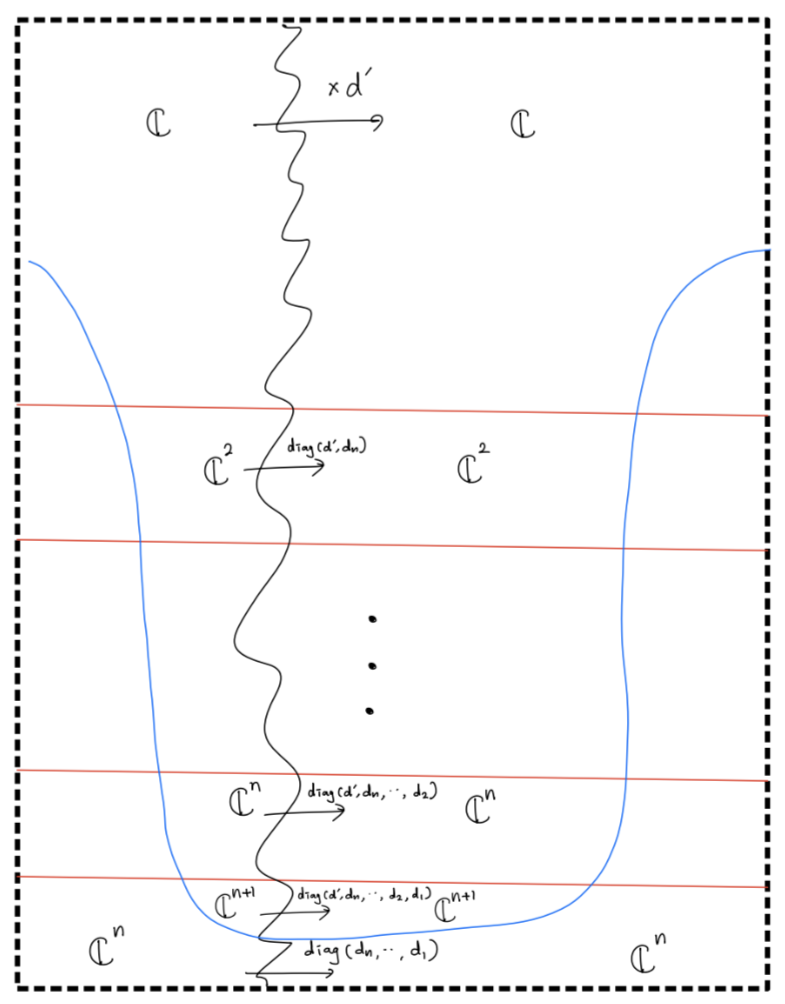
\includegraphics[scale = 0.95]{diagrams/cobord5/7.png}
    \caption{}
    \label{fig:your-label}
\end{figure}
\end{enumerate}
\end{enumerate}